\subsection{General principle}

% * * * * * * NEW FRAME * * * * * * %
\begin{frame}{Sending a transaction}
    \begin{center}
        \only<1>{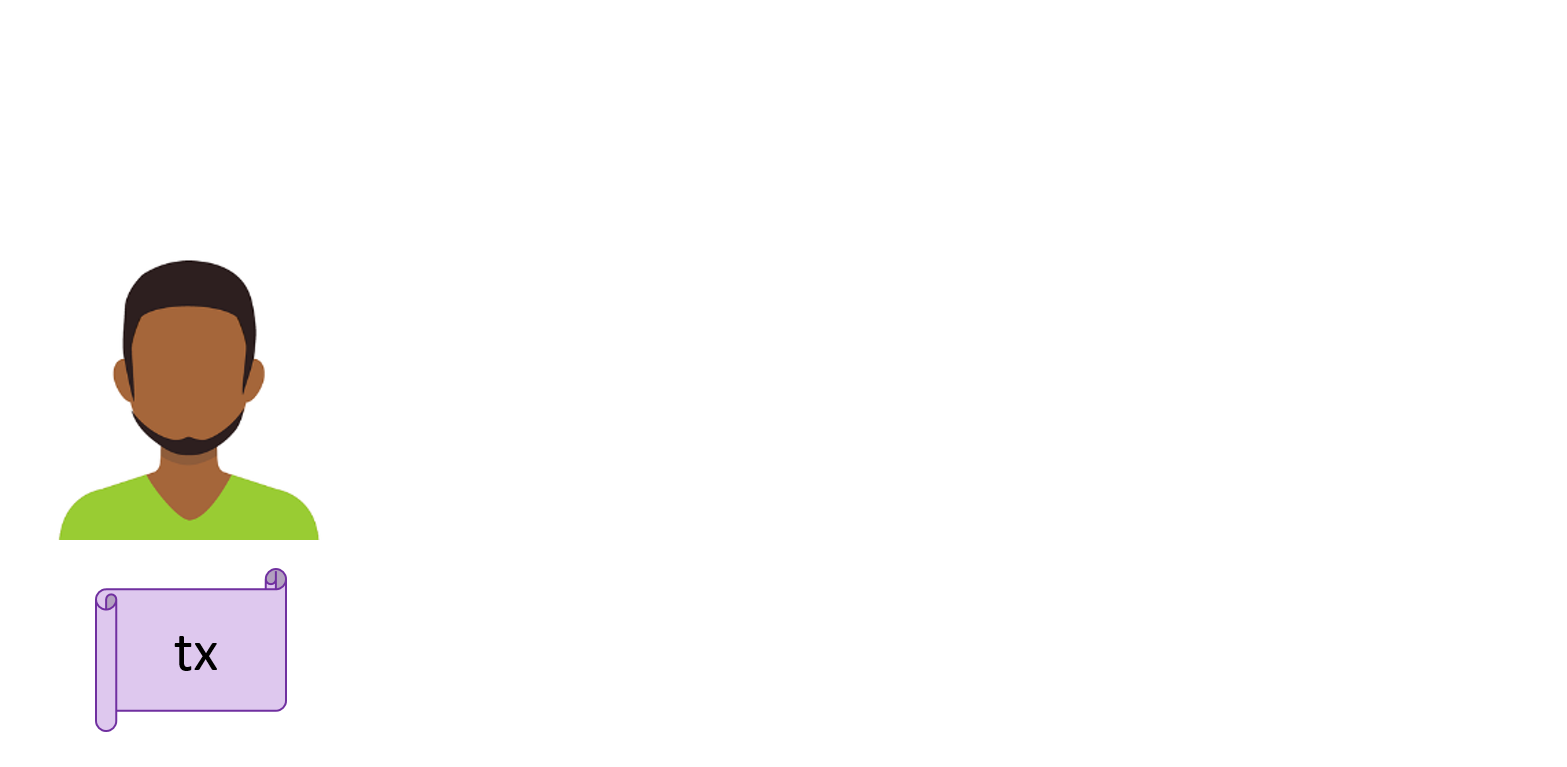
\includegraphics[scale=0.36]{Figures/BC_propagation_1.png}}
        \only<2>{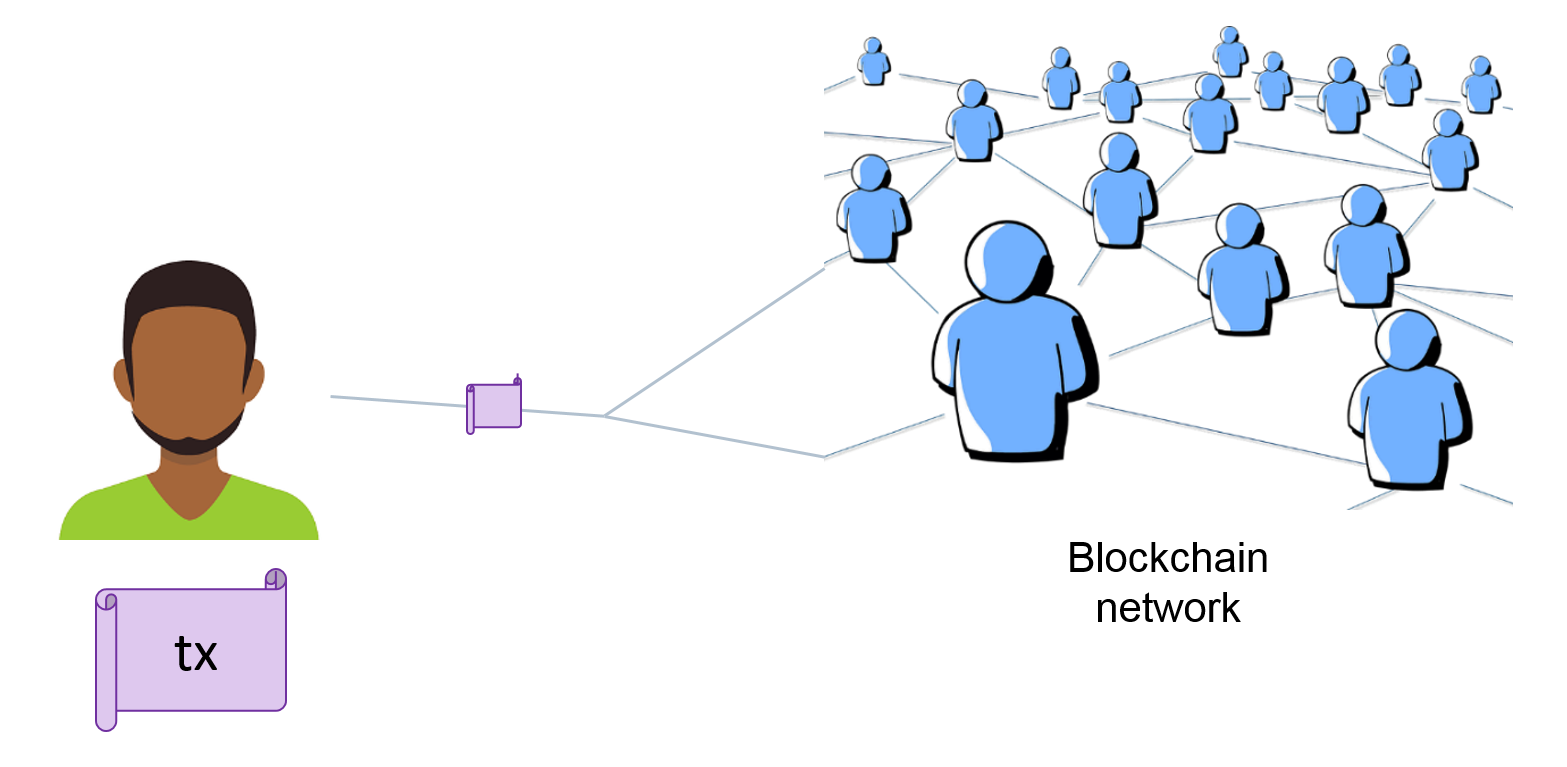
\includegraphics[scale=0.36]{Figures/BC_propagation_2.png}}  
        \only<3>{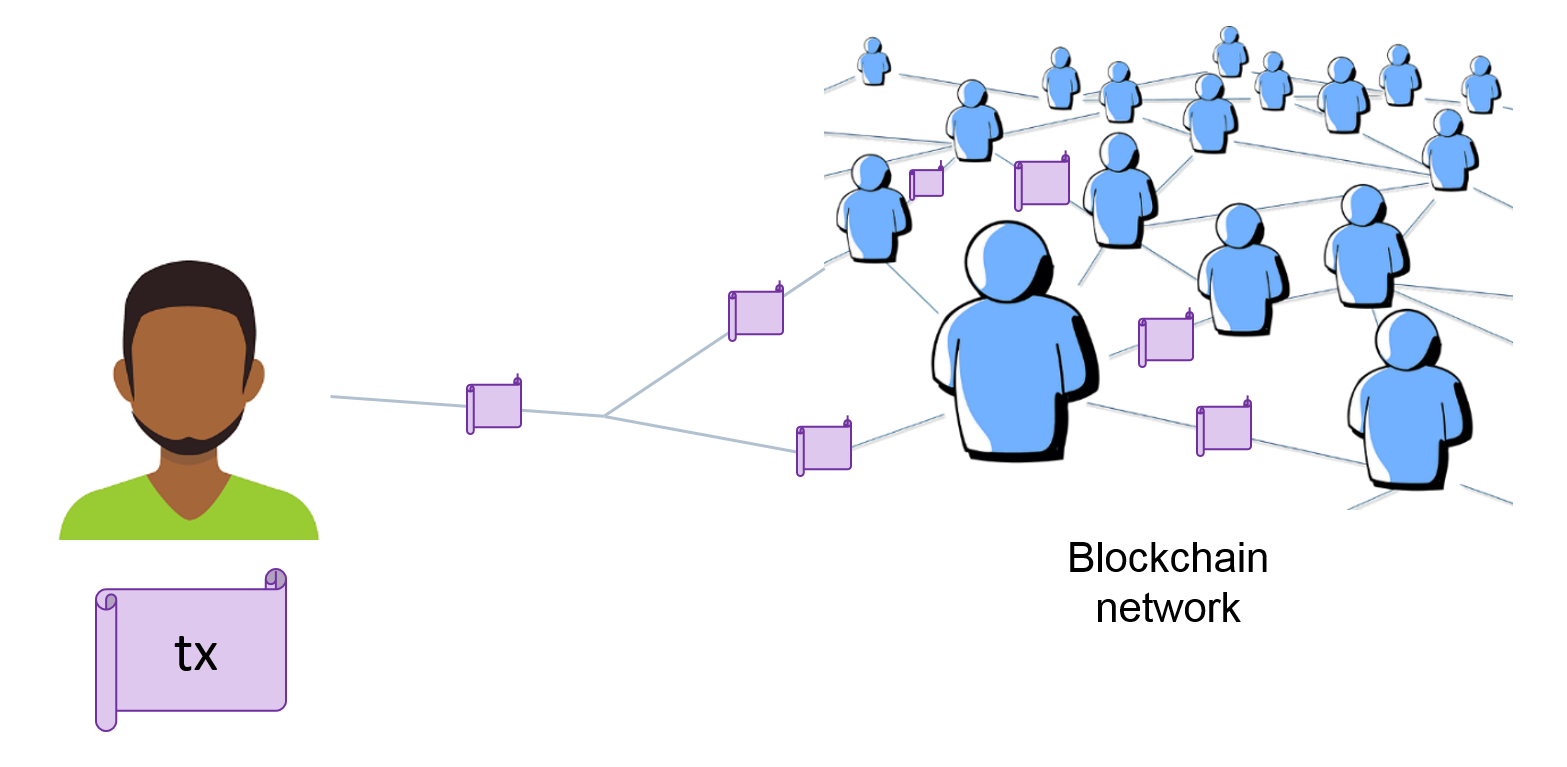
\includegraphics[scale=0.36]{Figures/BC_propagation_3.png}}
        \only<4>{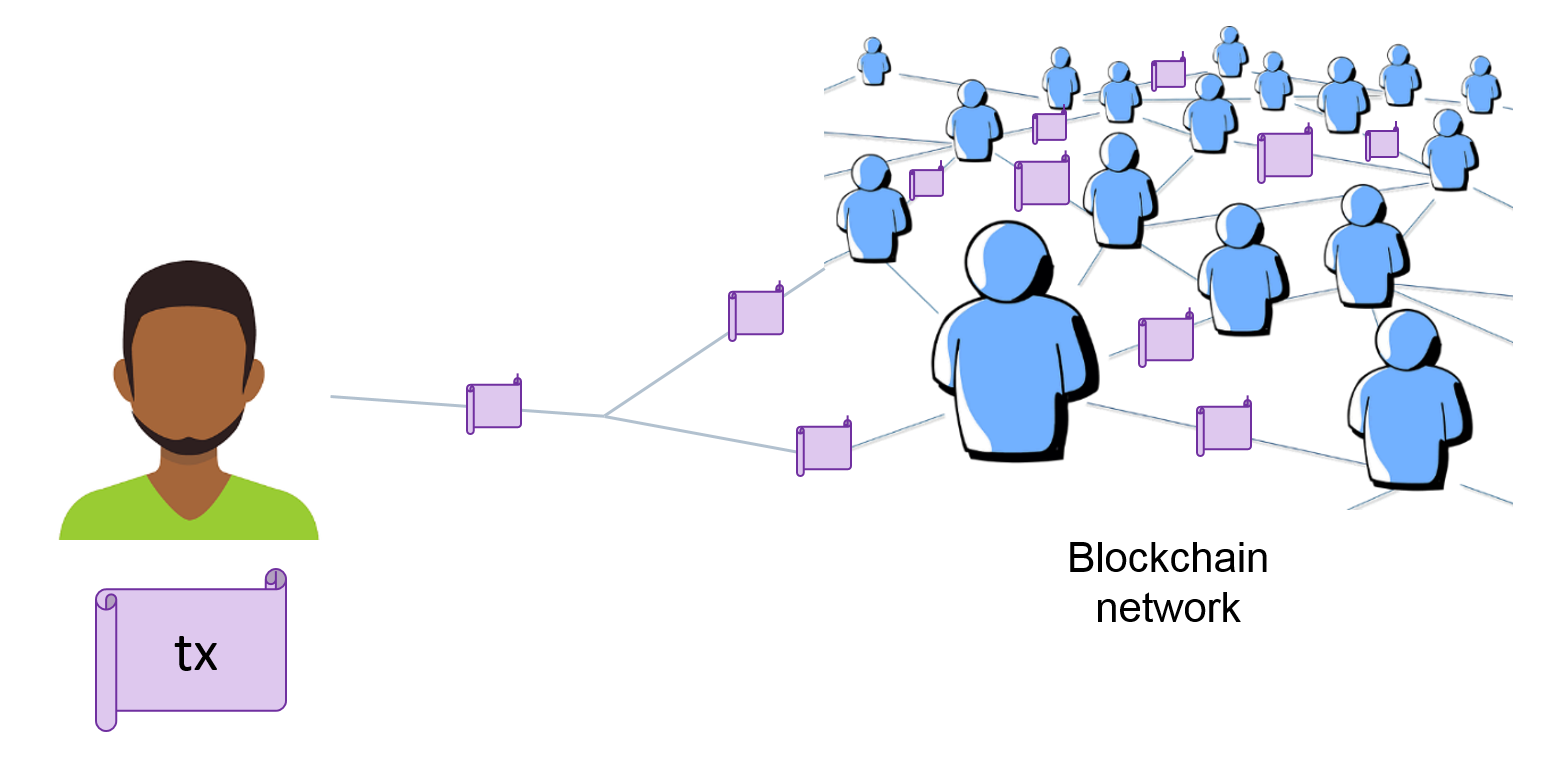
\includegraphics[scale=0.36]{Figures/BC_propagation_4.png}}
    \end{center}    
\end{frame}

% * * * * * * NEW FRAME * * * * * * %
\begin{frame}{Mining a block}
    \begin{center}
        \only<1>{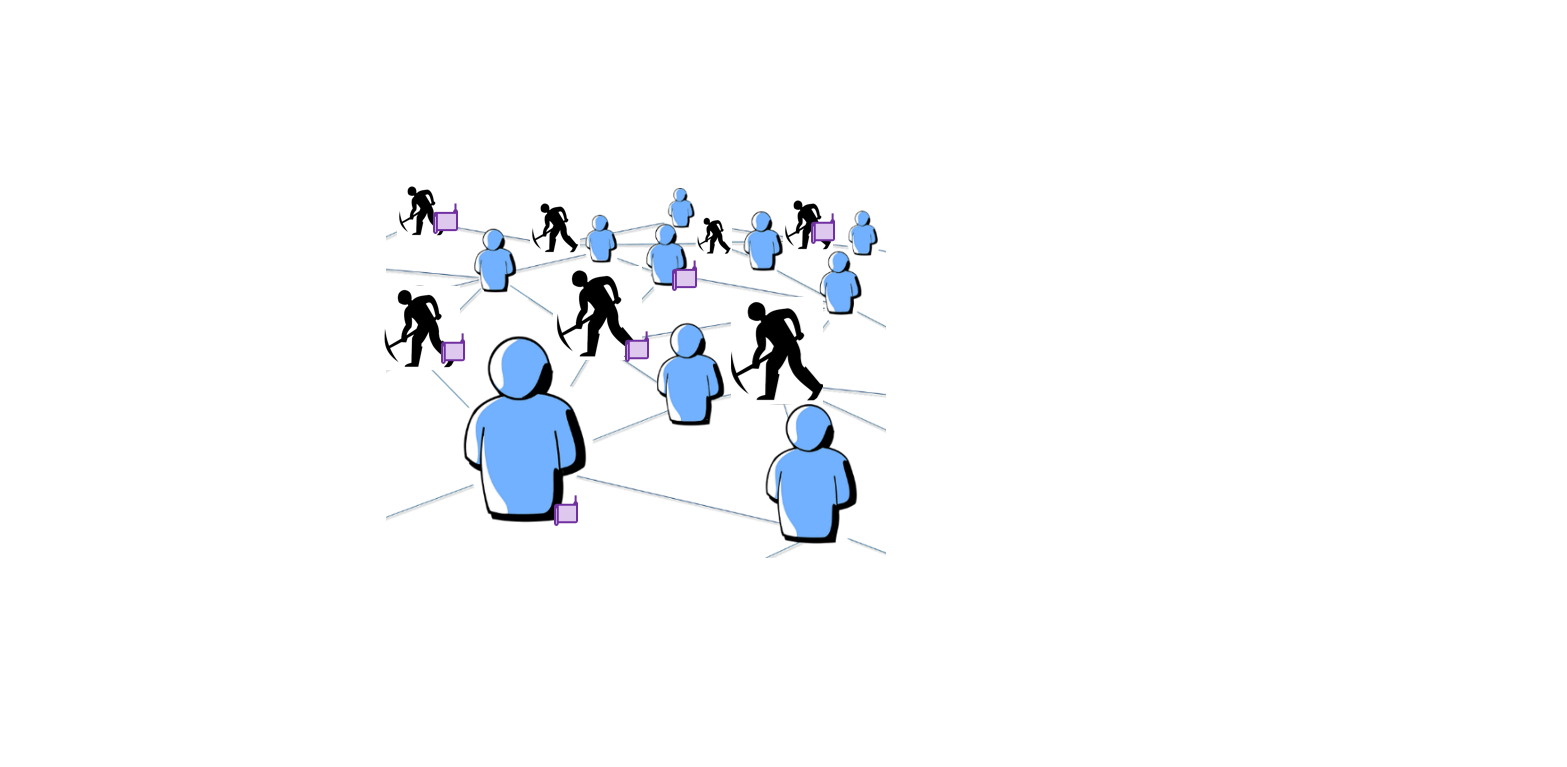
\includegraphics[scale=0.6]{Figures/BC_miners_1.png}}
        \only<2>{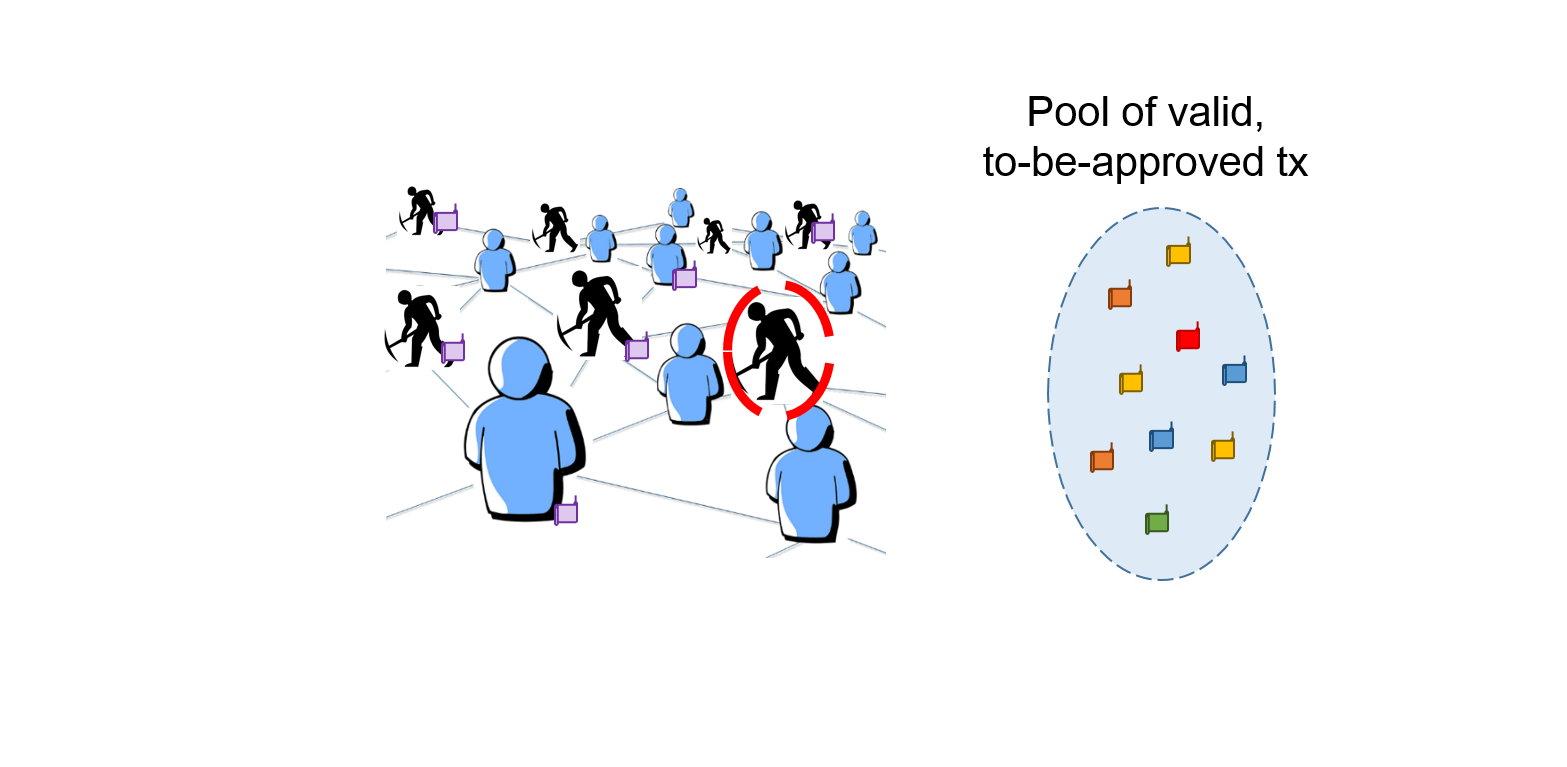
\includegraphics[scale=0.6]{Figures/BC_miners_2.png}}  
        \only<3>{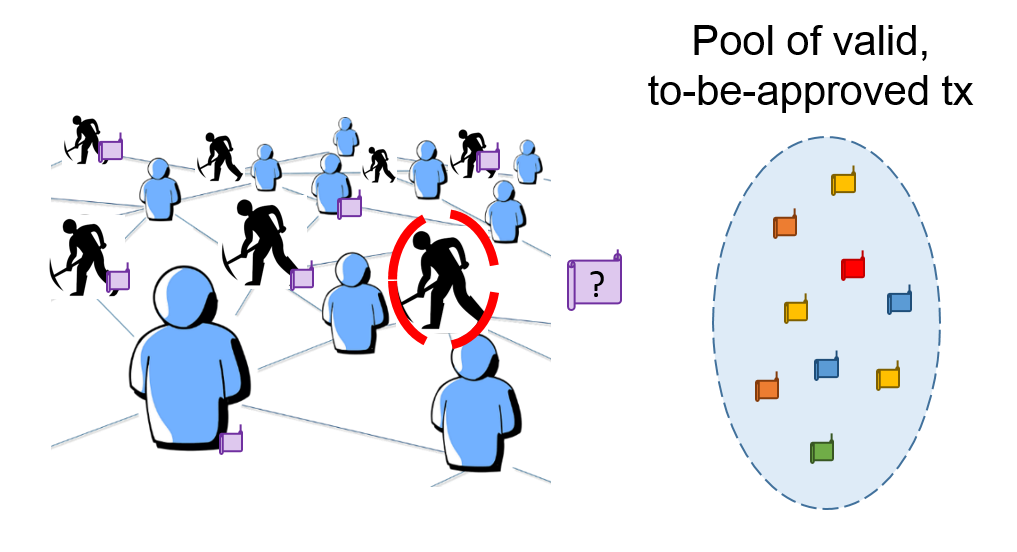
\includegraphics[scale=0.6]{Figures/BC_miners_3.png}}
        \only<4>{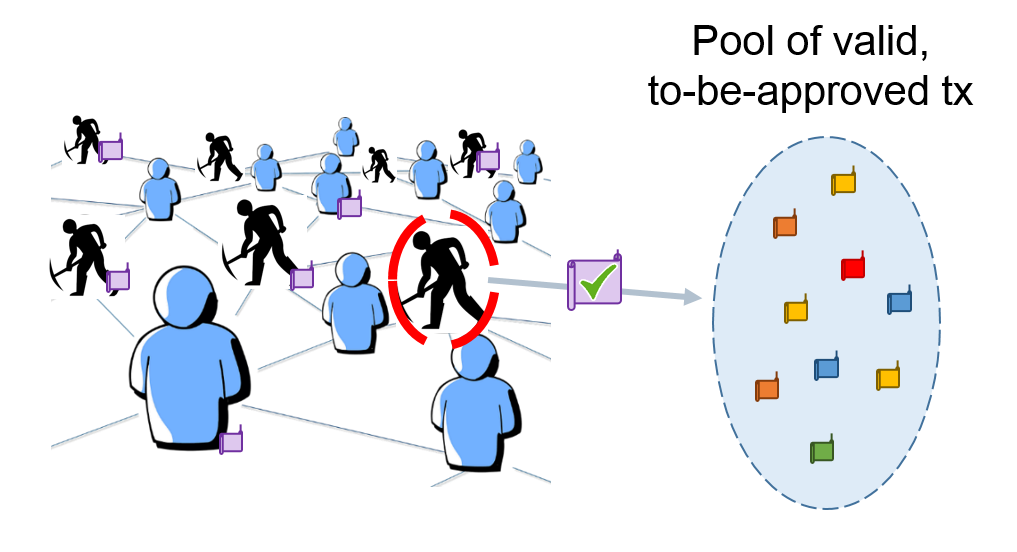
\includegraphics[scale=0.6]{Figures/BC_miners_4.png}}
        \only<5>{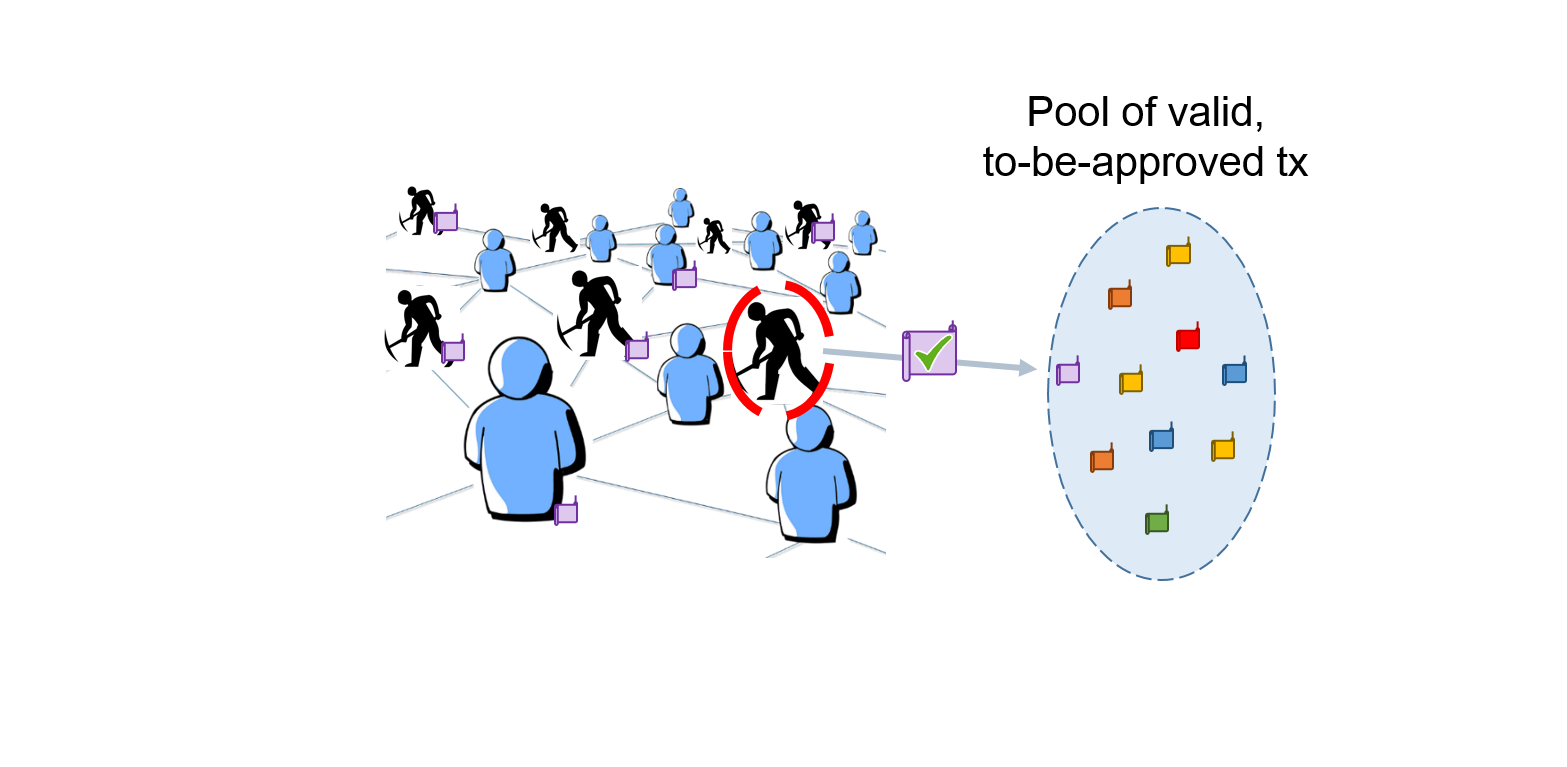
\includegraphics[scale=0.6]{Figures/BC_miners_5.png}}    
    \end{center}    
\end{frame}

% * * * * * * NEW FRAME * * * * * * %
\begin{frame}{Block dissemination}
    \begin{center}
        \only<1>{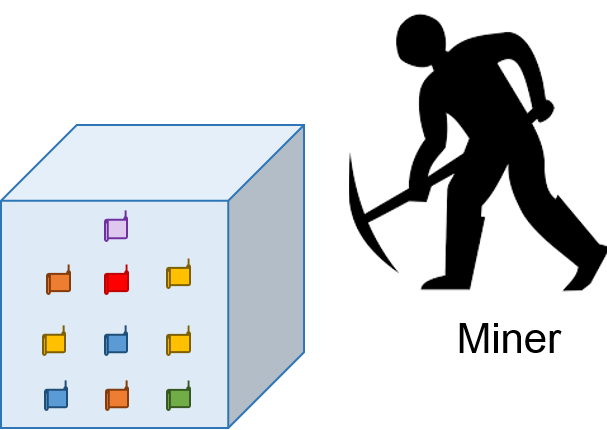
\includegraphics[scale=0.6]{Figures/bc_forged_1.png}}
        \only<2>{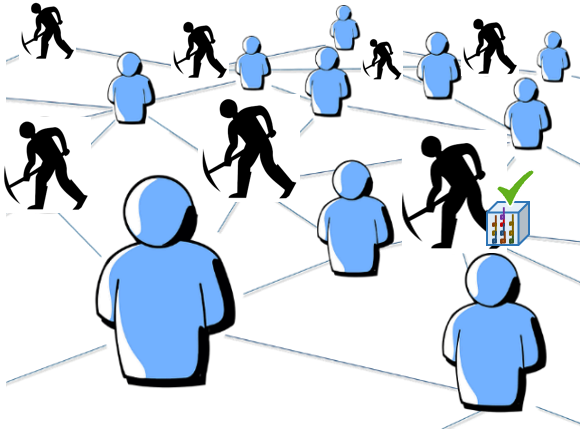
\includegraphics[scale=0.6]{Figures/bc_forged_2.png}}  
        \only<3>{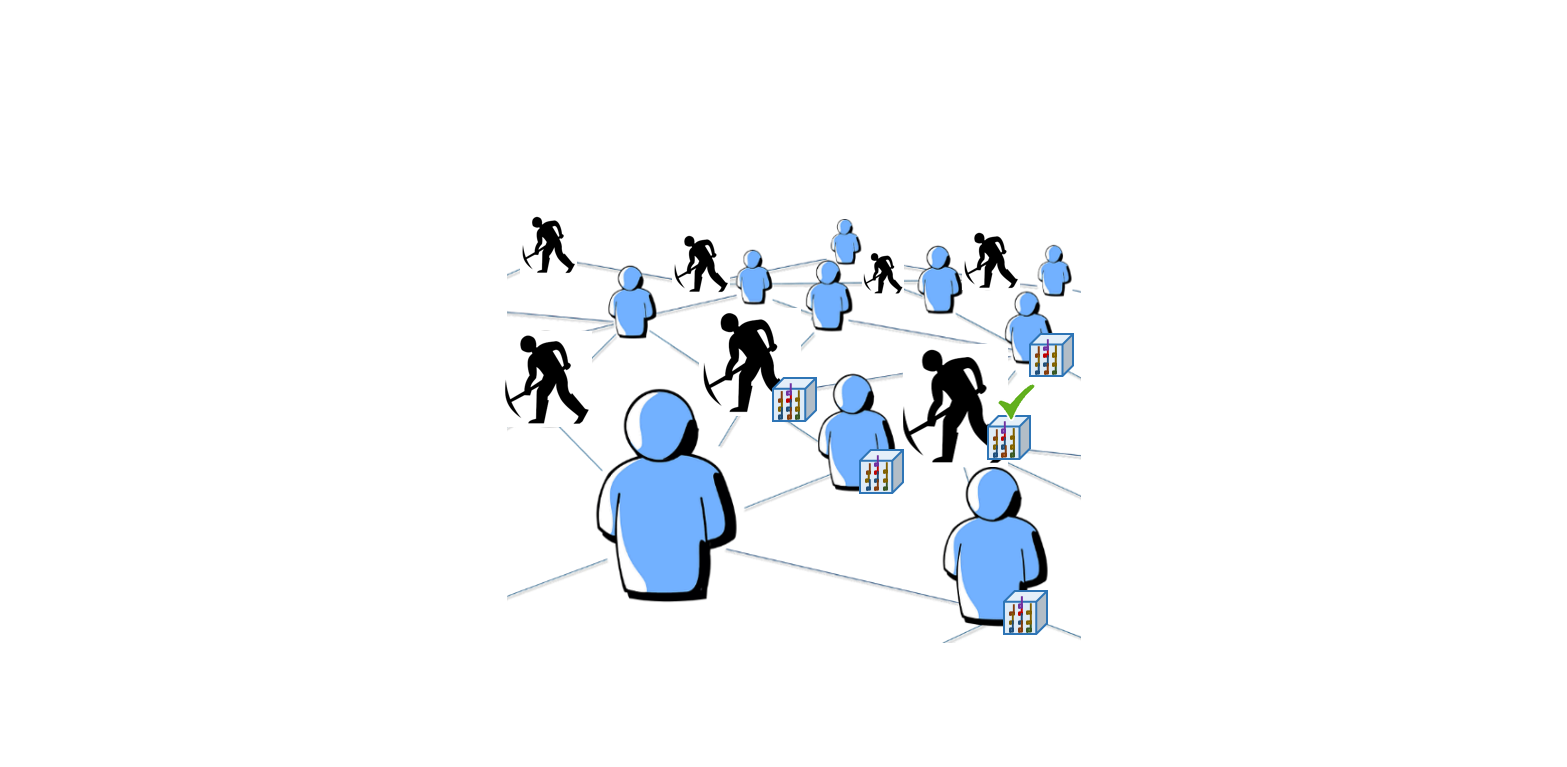
\includegraphics[scale=0.6]{Figures/bc_forged_3.png}}
        \only<4>{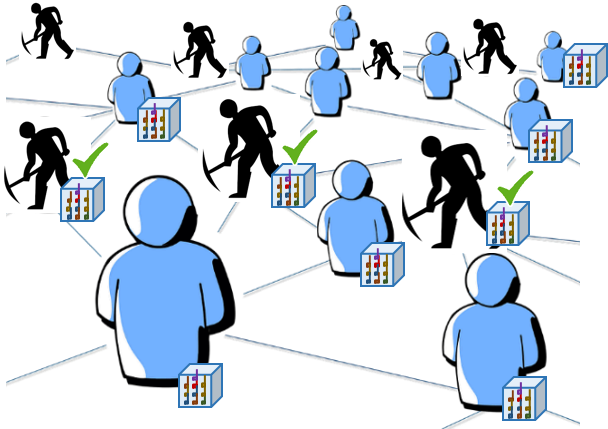
\includegraphics[scale=0.6]{Figures/bc_forged_4.png}}
    \end{center}    
\end{frame}

%
%% FRAME : TRANSACTIONS %%
\begin{frame}{Transactions}

\end{frame}

%% FRAME : ADDRESSES %%
\begin{frame}{Addresses}

\end{frame}

%% FRAME : MINERS %%
\begin{frame}{Miners}

\end{frame}

%% FRAME : BLOCKS %%
\begin{frame}{Blocks}

\end{frame}

%% FRAME : Smart contracts %%
\begin{frame}{Smart contracts}

\end{frame}

%% FRAME : Consensus %%
\begin{frame}{Consensus: Proof of Work}

\end{frame}

%% FRAME : Consensus %%
\begin{frame}{Consensus: Proof of Stake}

\end{frame}
\subsection{Basic Concepts}


%% FRAME : TRANSACTIONS %%
% \begin{frame}{Transactions}
%     \begin{center}
%         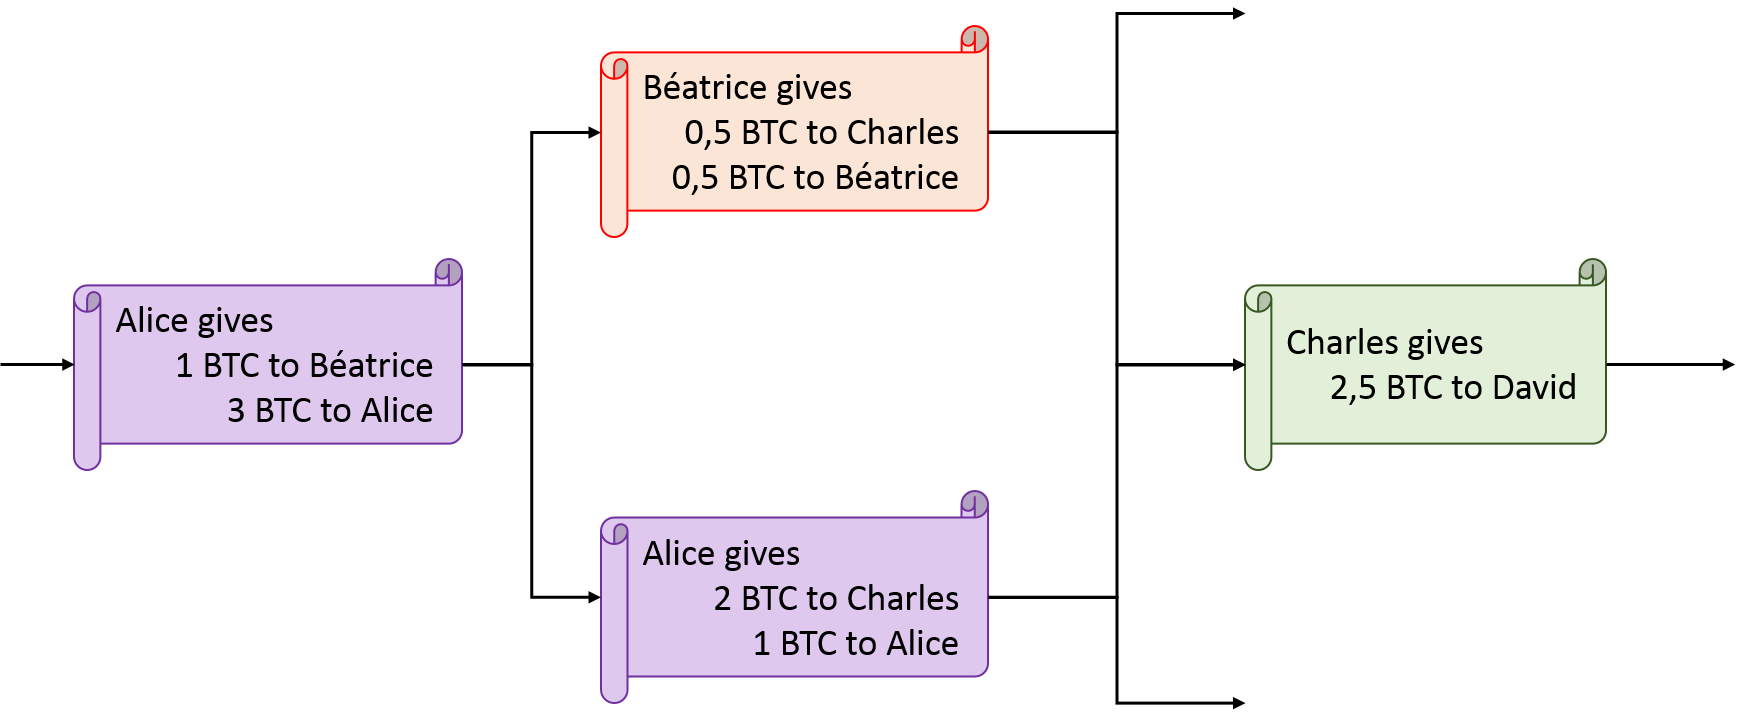
\includegraphics[scale=0.36]{Figures/tx.png}
%     \end{center}
% \end{frame}

%% FRAME : BLOCKS %%
\begin{frame}{Blocks}
    \begin{center}
        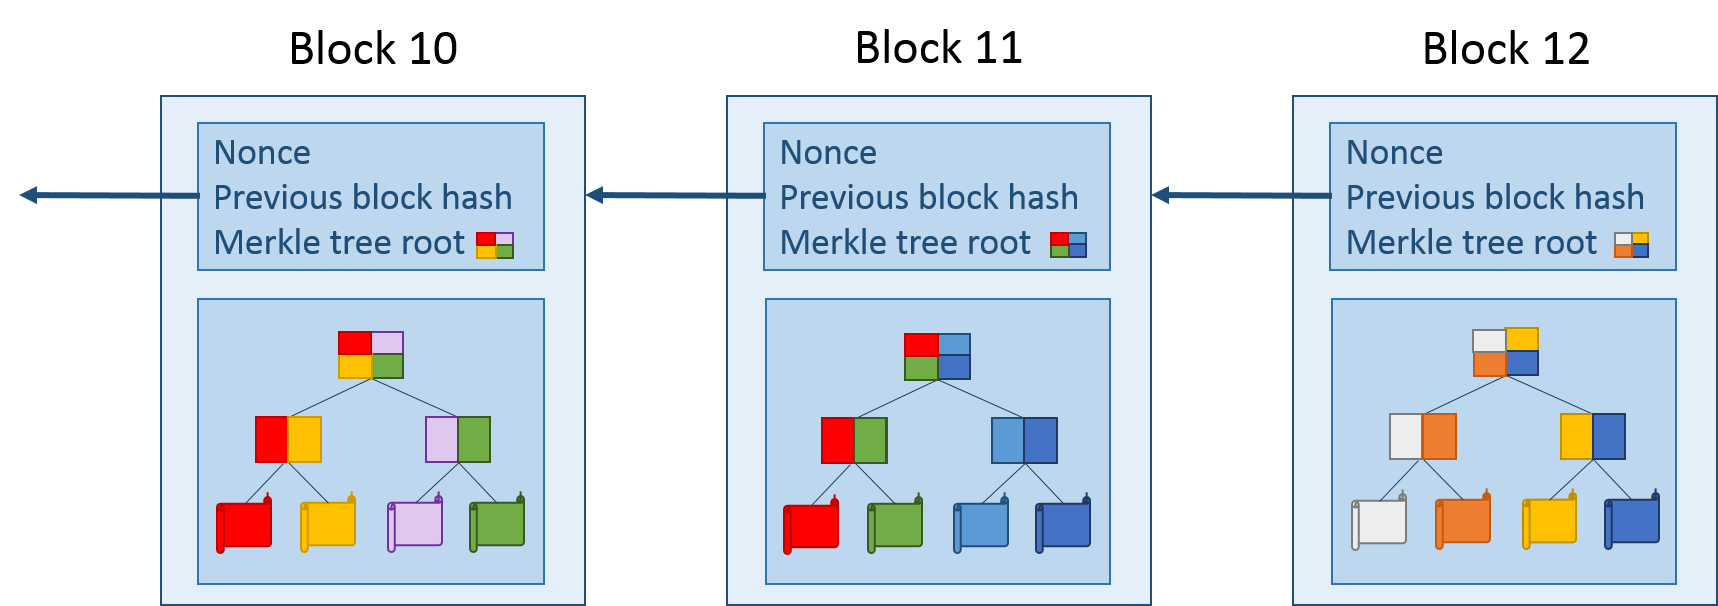
\includegraphics[scale=0.36]{Figures/blocks.png}
    \end{center}
\end{frame}

%% FRAME : Smart contracts %%
\begin{frame}{Smart contracts}
    \begin{center}
        \only<1>{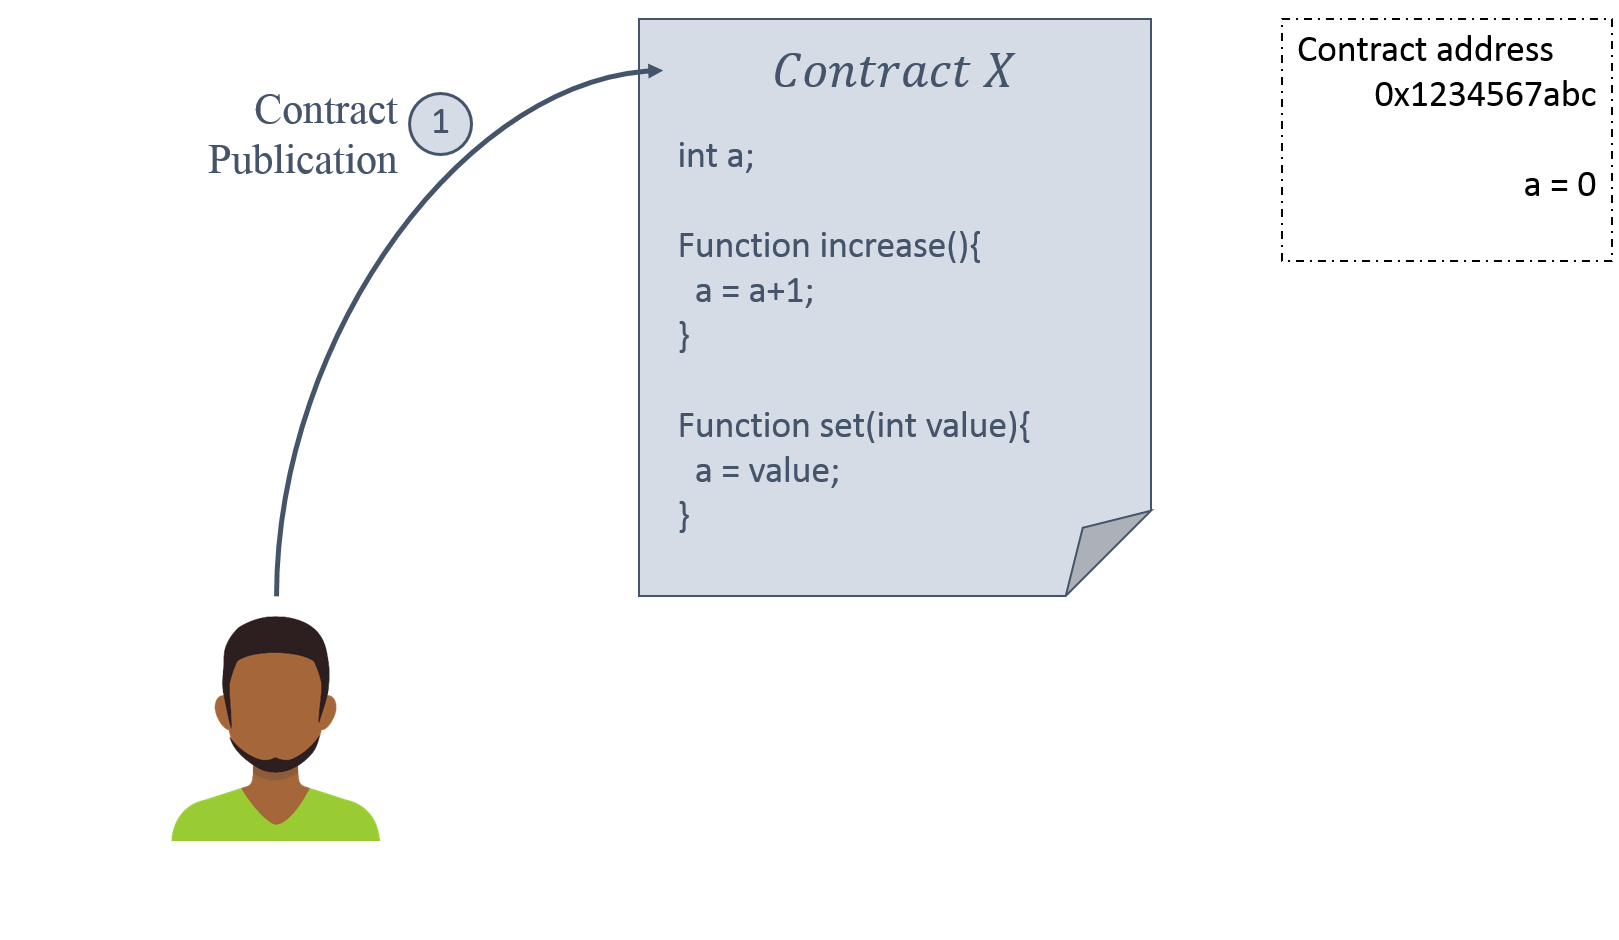
\includegraphics[scale=0.36]{Figures/bc_smart_contract_1.png}}
        \only<2>{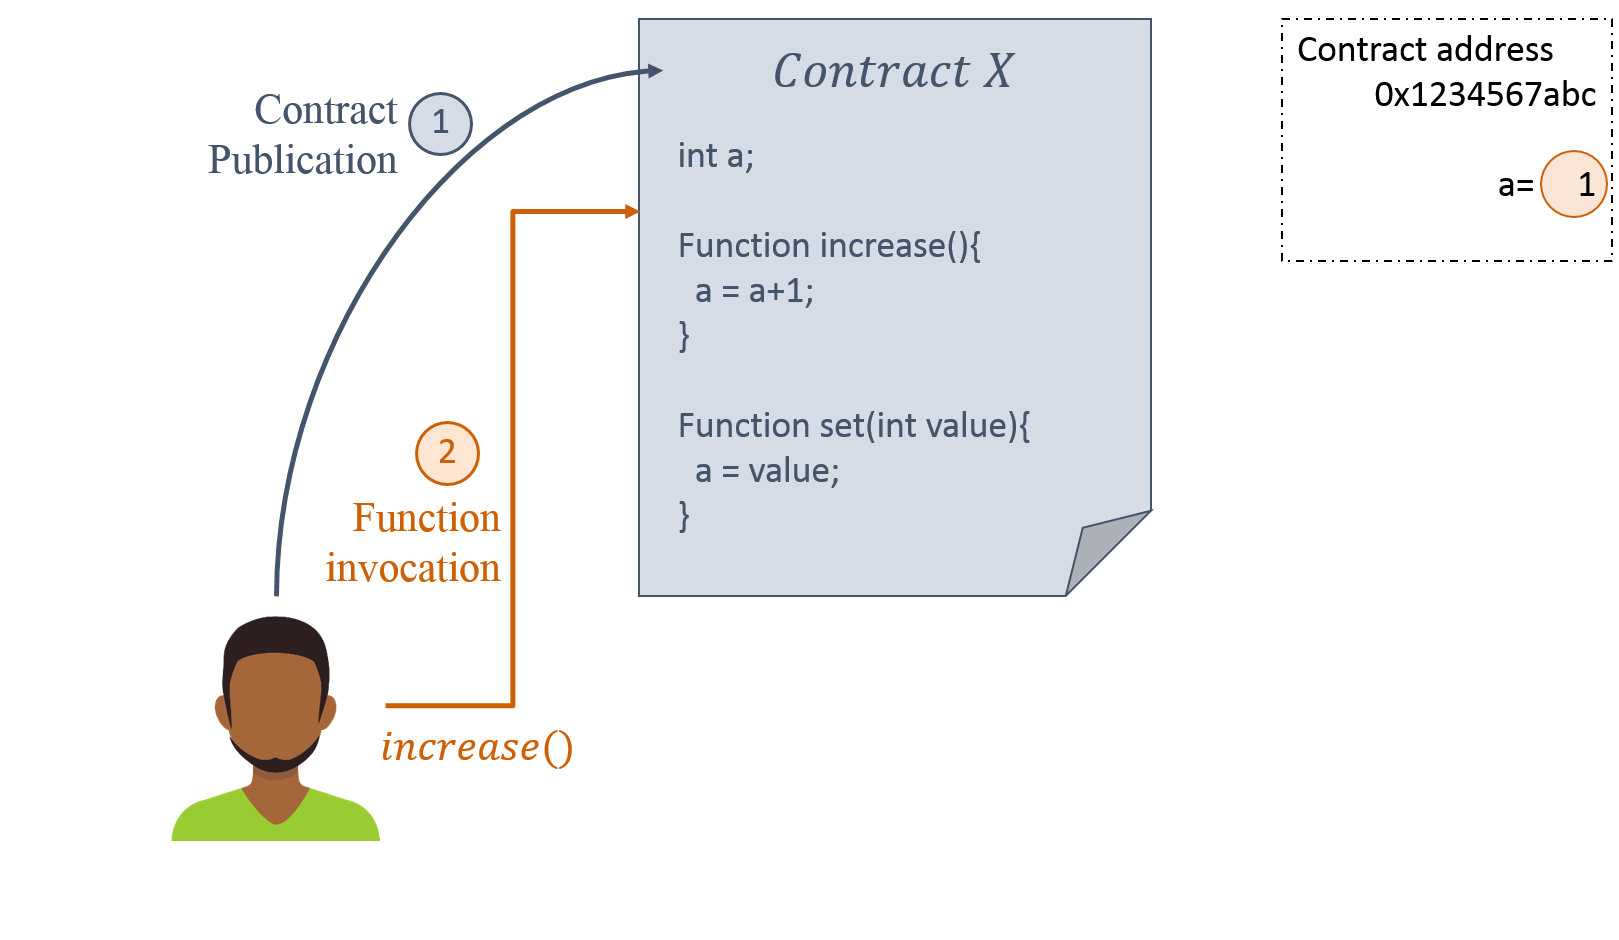
\includegraphics[scale=0.36]{Figures/bc_smart_contract_2.png}} 
        \only<3>{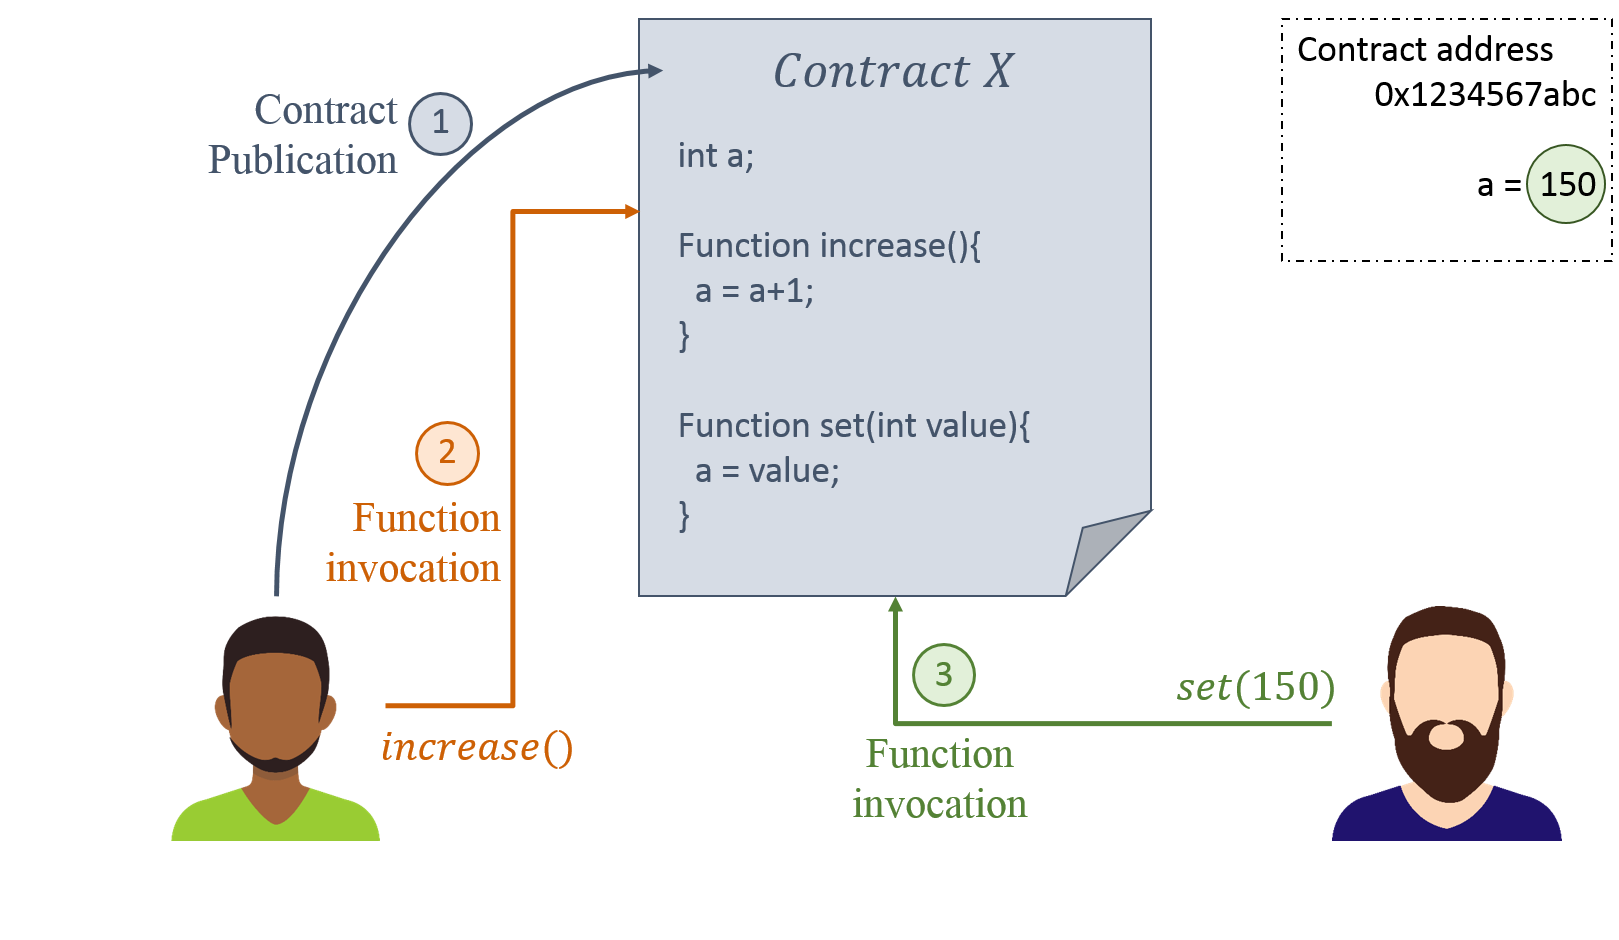
\includegraphics[scale=0.36]{Figures/bc_smart_contract_3.png}}
    \end{center}
\end{frame}

%% FRAME : ADDRESSES %%
\begin{frame}{Addresses}
    \begin{center}
        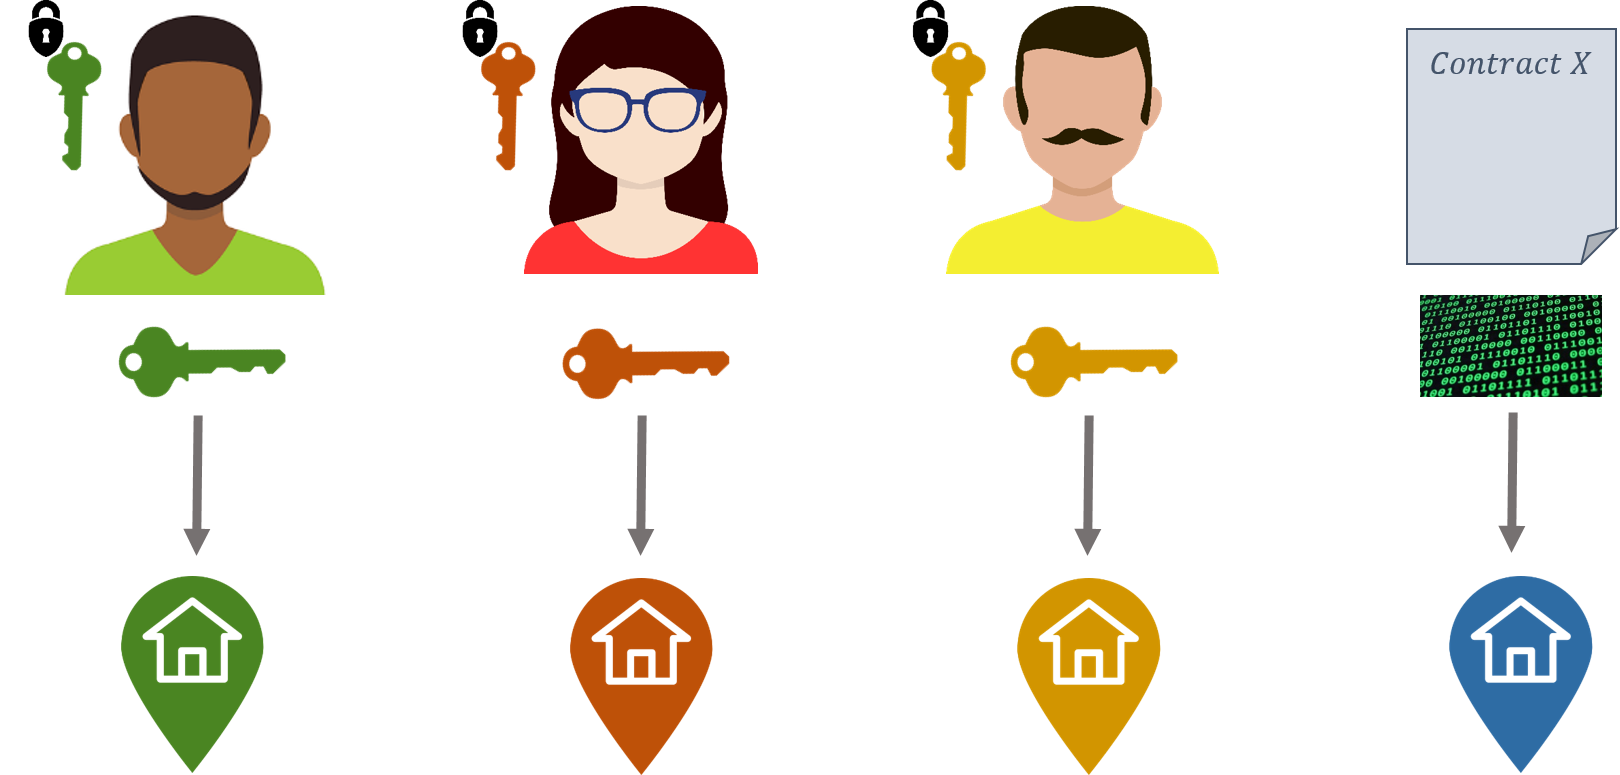
\includegraphics[scale=0.36]{Figures/BC_address.png}
    \end{center}
\end{frame}


%% FRAME : Consensus %%
\begin{frame}{Consensus protocol}
What it does:
    \begin{itemize}
        \item Orders transactions
        \item Bundles transactions into blocks
    \end{itemize}
\bigskip    
How it does it:
    \begin{itemize}
        \item Each miner work on \alert{their} block
        \item \alert{One} miner is \emph{selected}
        \item This miner's block is now the top of the chain
        \item Miners update their pool of tx 
        \item Miners accept the block by building on top of it
    \end{itemize}
\end{frame}

%% FRAME : Summury %%
\begin{frame}{Blockchain properties~\cite{pass2016analysis}}
A blockchain is a \alert{distributed} transaction-ordering system that has: 
    \begin{itemize}
        \item \textbf{Consistency over nodes} \newline Participants agree on a common history
        \item \textbf{Consistency over time} \newline The history cannot be modified
        \item \textbf{Growth} \newline New blocks are regularly added to the chain 
        \item \textbf{Plurality} \newline No one has a monopoly on mining blocks
    \end{itemize}
\end{frame}

\subsection{Challenges}

\subsubsection{Security}
\subsubsection{Governance}
\subsubsection{Limitation}